\documentclass[11pt,a4paper]{article}
\usepackage{amsmath,amssymb}
\usepackage{siunitx}
\usepackage[margin=2.5cm]{geometry}
\usepackage{graphicx}
\usepackage{booktabs}
\usepackage{xcolor}

\begin{document}

\noindent\textbf{\large Carrier Accumulation in GHz-Burst Femtosecond Excitation of Silicon}\\[4pt]
\noindent Burak Arayici \hfill \today

\bigskip

\section{The Problem: Unphysical Carrier Accumulation}

In the burst-mode excitation scheme, $N$ femtosecond pulses are delivered within a burst window $\tau_\text{burst}$. Each pulse generates free carriers via two-photon absorption (TPA). The free-carrier density evolves according to Eq.~5 of the manuscript:
\begin{equation}
\frac{dN_\text{fc}}{dt} = \frac{\beta I^2}{2\hbar\omega} - \frac{N_\text{fc}}{\tau_c}
\label{eq:rate}
\end{equation}
where $\beta$ is the TPA coefficient, $I$ is the pulse intensity, $\hbar\omega$ is the photon energy, and $\tau_c$ is the carrier lifetime.

Each femtosecond pulse generates a carrier density increment:
\begin{equation}
\Delta N_\text{fc} = \frac{\beta\, I_p^2\, \tau_p}{2\hbar\omega}
\label{eq:deltaN}
\end{equation}

With our parameters ($\beta = \SI{1.5e-11}{m/W}$, $I_p = \SI{1e16}{W/m^2}$ i.e.\ \SI{1}{TW/cm^2}, $\tau_p = \SI{100}{fs}$, $\hbar\omega = \SI{1.87e-19}{J}$):
\[
\Delta N_\text{fc} = \SI{4.0e26}{m^{-3}} \quad \text{per pulse}
\]

\subsection{Figure 1: No recombination}

If we neglect recombination entirely ($\tau_c \to \infty$), the carrier density after $k$ pulses is simply (Eq.~6 of the manuscript):
\begin{equation}
N_k = k \cdot \Delta N_\text{fc}
\label{eq:linear}
\end{equation}

This is a volumetric carrier density inside the silicon material itself --- no assumption about particle geometry or concentration is needed. Figure~1 plots $N_k$ vs.\ pulse number $k$ for $N = 1000$ pulses.

The key comparison is against the \textbf{silicon atomic density}:
\[
n_\text{Si} = \frac{8}{a^3} \approx \SI{5.0e28}{m^{-3}}
\]
where $a = \SI{5.431}{\angstrom}$ is the lattice constant of the diamond cubic structure (8 atoms per unit cell). The carrier density cannot physically exceed the number of atoms available to donate electrons.

\paragraph{At the focus.} All calculations use the Beer--Lambert attenuated intensity at $z = \SI{500}{\mu m}$ (see Section~1.2 for the BL derivation):
\[
\Delta N_\text{fc}^\text{(focus)} = \frac{\beta\,I_\text{focus}^2\,\tau_p}{2\hbar\omega} = \SI{1.4e24}{m^{-3}} \quad \text{per pulse}
\]
After $k = 1000$ pulses with no recombination: $N_{1000} = \SI{1.4e27}{m^{-3}}$ ($0.03 \times n_\text{Si}$). At the focus the no-recombination model remains below $n_\text{Si}$, but gives a carrier density that grows without bound --- the question is how much recombination reduces it further.

\begin{figure}[h]
\centering
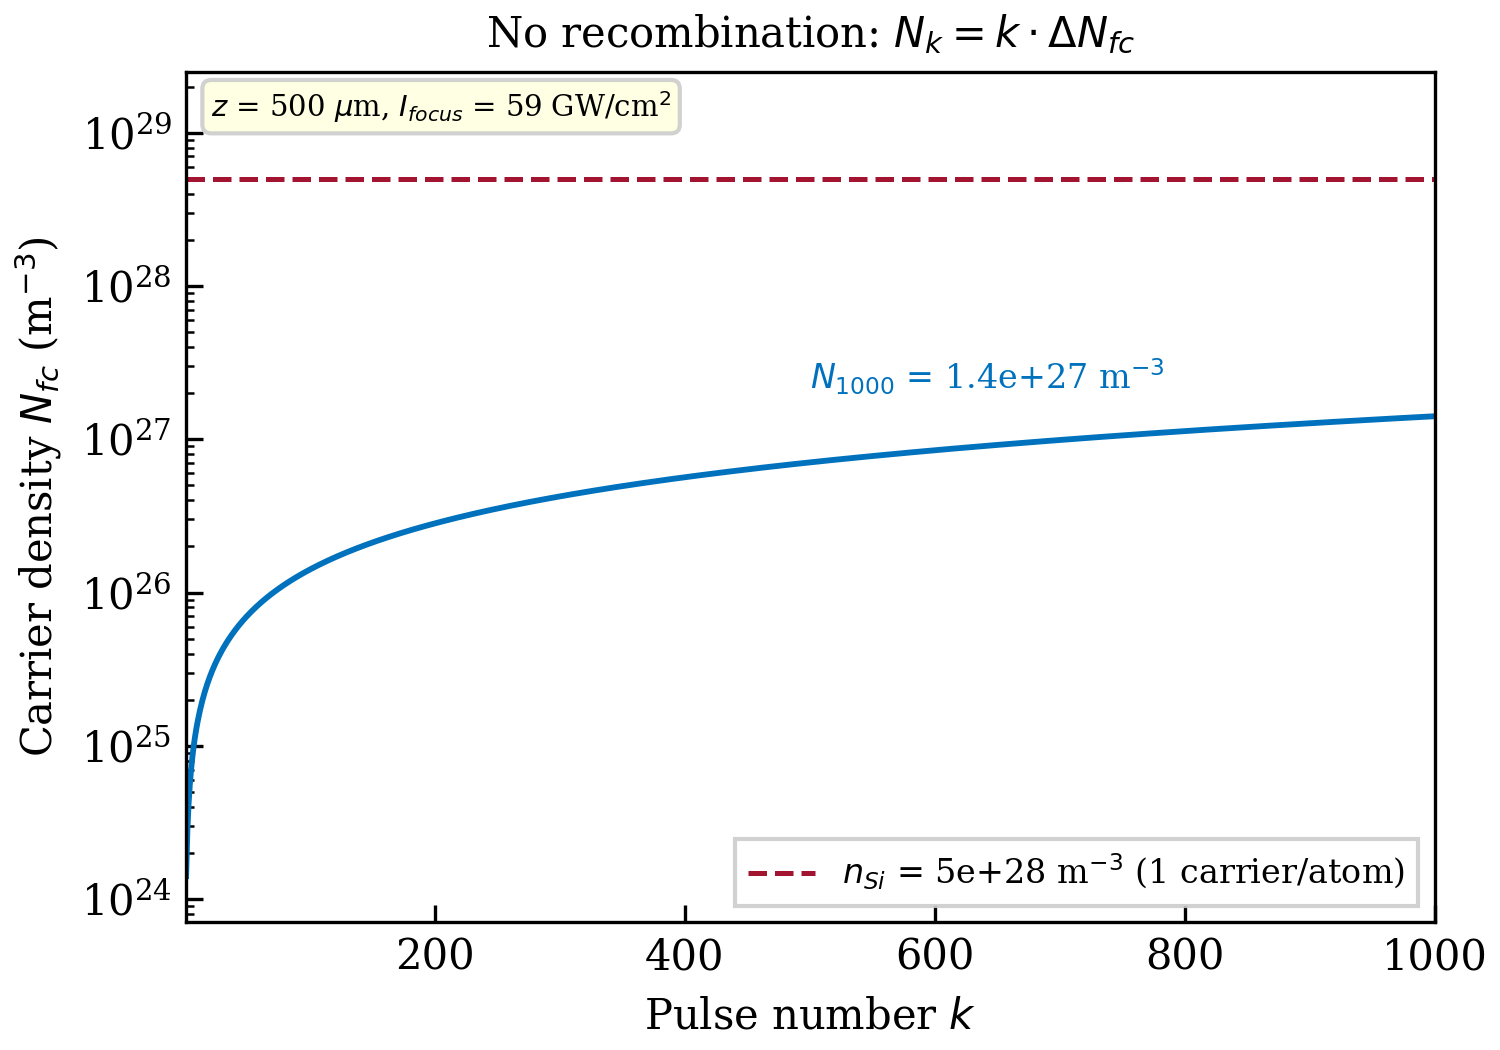
\includegraphics[width=0.75\textwidth]{figures_email/fig1_no_recombination.png}
\caption{Carrier density vs.\ pulse number with no recombination at the focus ($z = \SI{500}{\mu m}$, $I_\text{focus} = \SI{59}{GW/cm^2}$). Without any recombination mechanism, carriers accumulate linearly to $N_{1000} = \SI{1.4e27}{m^{-3}}$.}
\label{fig:no_recomb}
\end{figure}


\newpage
\subsection{Figure 2: Full solution of Eq.~5 with pulsed excitation}

The source term in Eq.~\eqref{eq:rate} is not constant --- it is a periodic step function. The laser is on (at intensity $I$) for duration $\tau_p$, then off for the inter-pulse gap $(\tau_r - \tau_p)$:
\[
G(t) = \begin{cases} G = \dfrac{\beta I^2}{2\hbar\omega} & \text{during pulse} \\[6pt] 0 & \text{between pulses} \end{cases}
\]

\paragraph{During the pulse} ($0 < t < \tau_p$): The ODE is $dN/dt + N/\tau_c = G$, a first-order linear ODE. Using the integrating factor $\mu = e^{t/\tau_c}$:
\[
\frac{d}{dt}\!\left[N\,e^{t/\tau_c}\right] = G\,e^{t/\tau_c}
\]
Integrating with initial condition $N(0) = N_0$ (carrier density at the start of the pulse):
\begin{equation}
N(t) = G\,\tau_c\!\left(1 - e^{-t/\tau_c}\right) + N_0\,e^{-t/\tau_c}
\label{eq:during_pulse}
\end{equation}
At the end of the pulse ($t = \tau_p$):
\begin{equation}
N_+ = G\,\tau_c\!\left(1 - e^{-\tau_p/\tau_c}\right) + N_0\,e^{-\tau_p/\tau_c}
\label{eq:N_after_pulse}
\end{equation}

\paragraph{Between pulses} ($\tau_p < t < \tau_r$): No generation, pure decay:
\begin{equation}
N(t) = N_+\,e^{-(t - \tau_p)/\tau_c}
\label{eq:between_pulses}
\end{equation}
At $t = \tau_r$ (just before the next pulse):
\[
N(\tau_r) = N_+\,e^{-(\tau_r - \tau_p)/\tau_c}
\]

\paragraph{Steady-state condition.} In steady state, the carrier density must be periodic: $N(\tau_r) = N_0$. Substituting Eq.~\eqref{eq:N_after_pulse}:
\[
N_0 = \left[G\,\tau_c\!\left(1 - e^{-\tau_p/\tau_c}\right) + N_0\,e^{-\tau_p/\tau_c}\right] e^{-(\tau_r - \tau_p)/\tau_c}
\]
Noting that $e^{-\tau_p/\tau_c} \cdot e^{-(\tau_r - \tau_p)/\tau_c} = e^{-\tau_r/\tau_c}$:
\[
N_0\!\left(1 - e^{-\tau_r/\tau_c}\right) = G\,\tau_c\!\left(1 - e^{-\tau_p/\tau_c}\right) e^{-(\tau_r - \tau_p)/\tau_c}
\]
\begin{equation}
\boxed{N_0 = \frac{G\,\tau_c\!\left(1 - e^{-\tau_p/\tau_c}\right) e^{-(\tau_r - \tau_p)/\tau_c}}{1 - e^{-\tau_r/\tau_c}}}
\label{eq:N0_exact}
\end{equation}
The peak density (right after a pulse) is:
\begin{equation}
N_\text{peak} = N_0\,e^{-\tau_p/\tau_c} + G\,\tau_c\!\left(1 - e^{-\tau_p/\tau_c}\right)
\label{eq:Npeak_exact}
\end{equation}

\paragraph{Simplification.} Since $\tau_p = \SI{100}{fs} \ll \tau_c = \SI{300}{ps}$, we have $e^{-\tau_p/\tau_c} \approx 1$ and $1 - e^{-\tau_p/\tau_c} \approx \tau_p/\tau_c$, so:
\[
N_\text{peak} \approx \frac{G\,\tau_p}{1 - e^{-\tau_r/\tau_c}} = \frac{\Delta N_\text{fc}}{1 - e^{-\tau_r/\tau_c}}
\]
which recovers the discrete pulse-by-pulse result.

\paragraph{Intensity at the focus.} The focal intensity $I_p$ is set by the pulse energy, pulse duration, and focusing optics. With $F_p = \SI{0.1}{J/cm^2}$ and $\tau_p = \SI{100}{fs}$:
\[
I_p = \frac{F_p}{\tau_p} = \SI{1e16}{W/m^2} \quad (\SI{1}{TW/cm^2})
\]

\paragraph{Beer--Lambert attenuation.} In tissue, the intensity at focal depth $z$ is:
\[
I(z) = I_p\,e^{-\mu_t\,z}
\]
where $\mu_t = \mu_a + \mu_s = \SI{5650}{m^{-1}}$ \cite{yaroslavsky2002}. At $z = \SI{500}{\mu m}$:
\[
I_\text{focus} = 0.059\,I_p = \SI{5.9e14}{W/m^2} \quad (\SI{59}{GW/cm^2})
\]
The per-pulse carrier generation at the focus:
\[
\Delta N_\text{fc}^\text{(focus)} = \frac{\beta\,I_\text{focus}^2\,\tau_p}{2\hbar\omega} = \SI{1.4e24}{m^{-3}}
\]
The steady-state peak density:
\[
N_\text{peak} = \frac{\SI{1.4e24}{}}{1 - e^{-1/300}} = \SI{4.2e26}{m^{-3}} \quad (0.008 \times n_\text{Si})
\]
This is well below $n_\text{Si}$ --- the combination of Beer--Lambert attenuation and the correct pulsed duty cycle ($\tau_p/\tau_r = 0.1$) keeps the carrier density physical at this depth.

\begin{figure}[h]
\centering
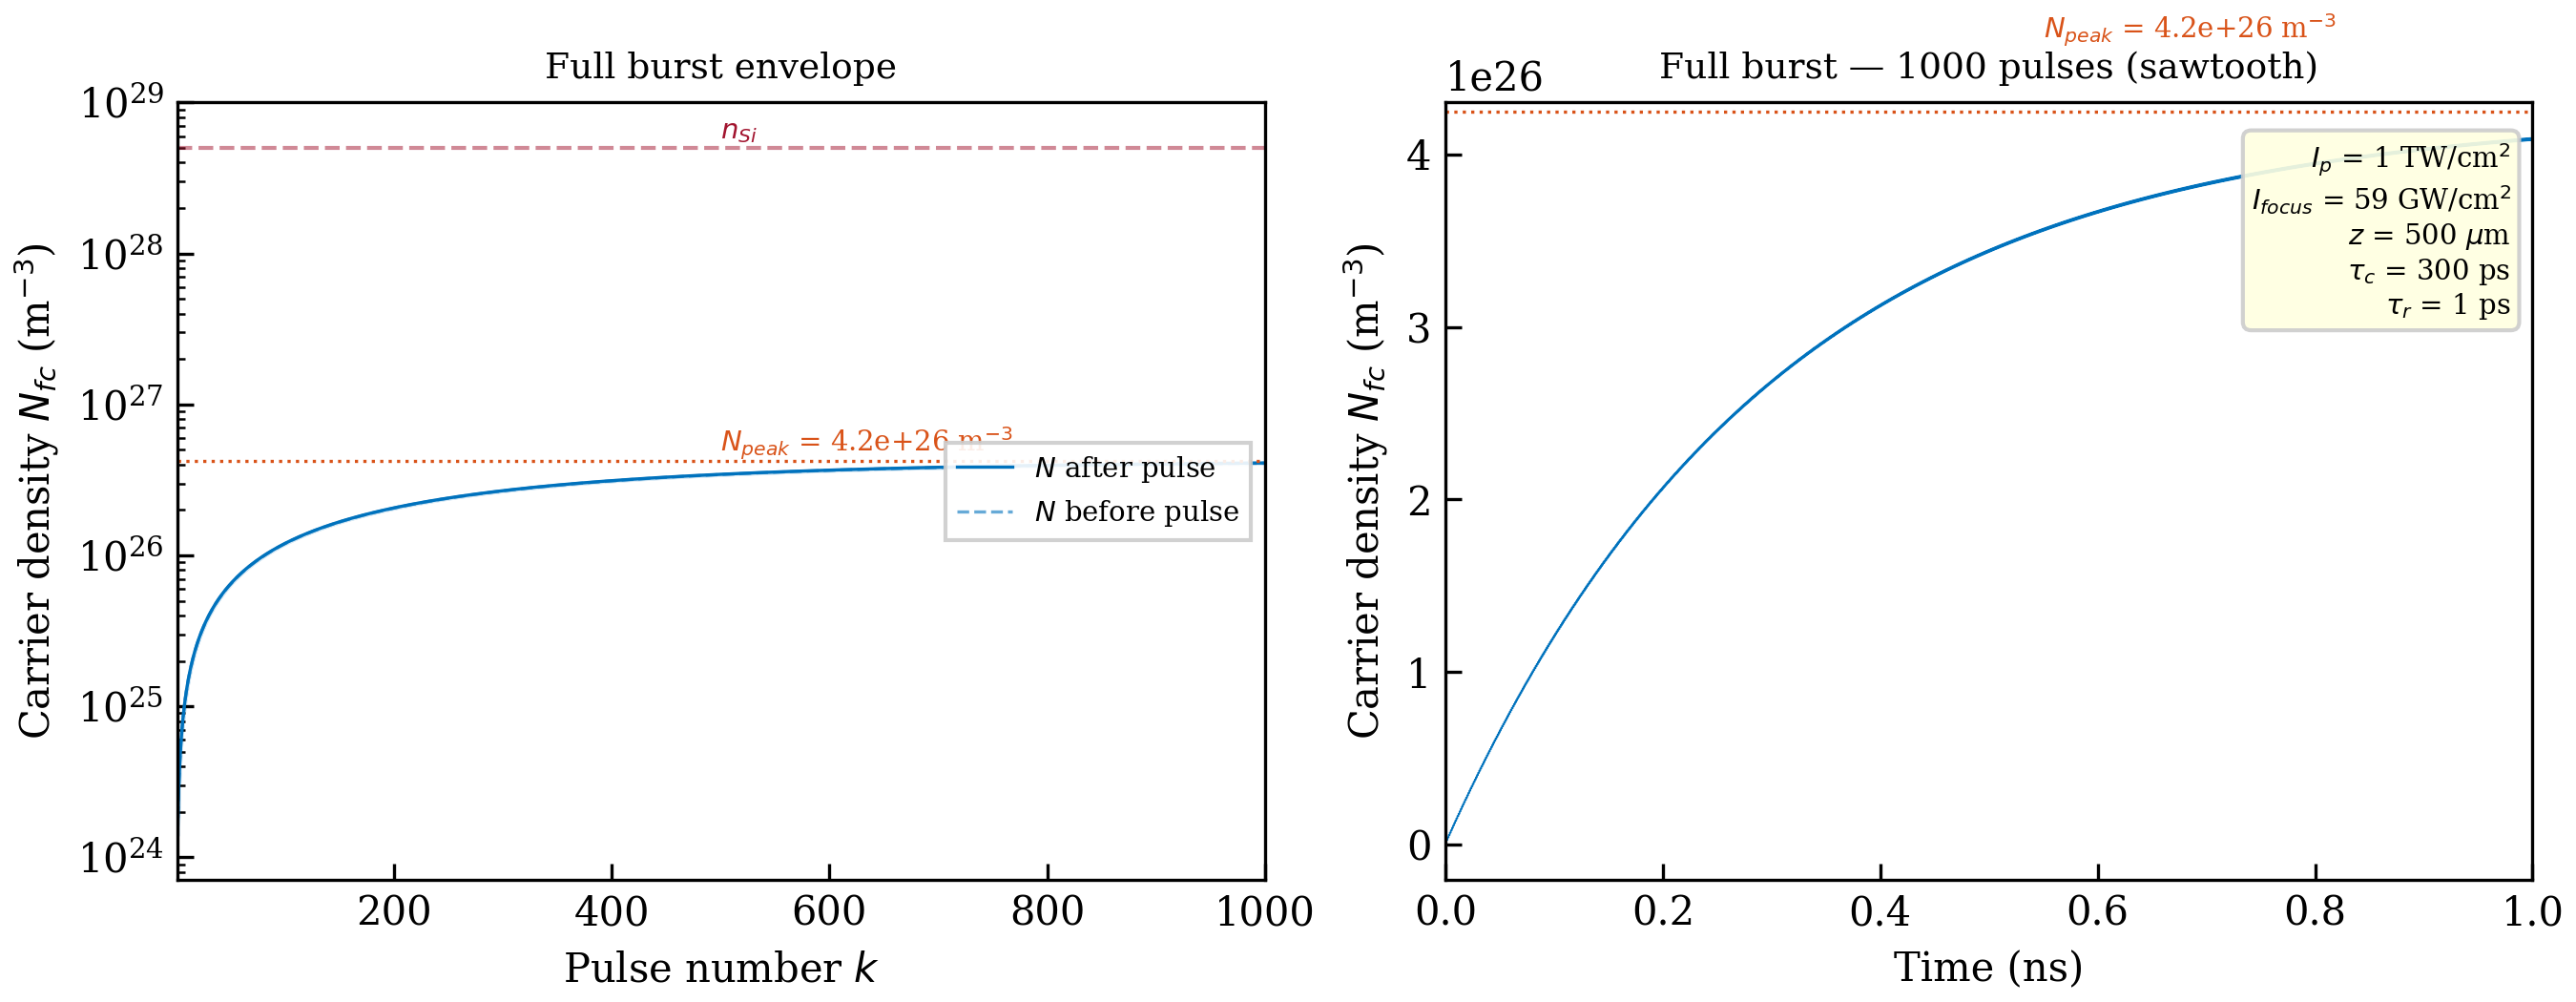
\includegraphics[width=0.75\textwidth]{figures_email/fig2b_continuous_ode.png}
\caption{Pulsed ODE solution at the focus ($z = \SI{500}{\mu m}$, $I_\text{focus} = \SI{59}{GW/cm^2}$). The carrier density shows the sawtooth build-up and inter-pulse decay, reaching a steady-state peak of $N_\text{peak} = \SI{4.2e26}{m^{-3}}$.}
\label{fig:pulsed_ode}
\end{figure}


\newpage
\section{Adding Auger Recombination}

We simply add one term to Eq.~\eqref{eq:rate}:
\begin{equation}
\frac{dN}{dt} = \frac{\beta I^2}{2\hbar\omega} - \frac{N}{\tau_c} - C\,N^3
\label{eq:auger_ode}
\end{equation}
where $C = \SI{3.8e-31}{cm^6/s}$ is the Auger coefficient for c-Si \cite{dziewior1977}. The only change is the $CN^3$ term.

\paragraph{Between pulses} ($G = 0$): the ODE becomes:
\begin{equation}
\frac{dN}{dt} = -\frac{N}{\tau_c} - C\,N^3
\label{eq:bernoulli}
\end{equation}
This is a Bernoulli equation. We solve it by substituting $u = N^{-2}$, which gives $du/dt = -2\,N^{-3}\,dN/dt$:
\[
\frac{du}{dt} = \frac{2u}{\tau_c} + 2C
\]
This is linear in $u$ and solvable with the integrating factor $e^{-2t/\tau_c}$:
\[
u(t) = \left(u_0 + C\,\tau_c\right) e^{2t/\tau_c} - C\,\tau_c
\]
Substituting back $u = 1/N^2$ with initial condition $N(0) = N_0$:
\begin{equation}
\boxed{N(t) = \frac{1}{\sqrt{\left(\dfrac{1}{N_0^2} + C\,\tau_c\right) e^{2t/\tau_c} - C\,\tau_c}}}
\label{eq:bernoulli_solution}
\end{equation}

\paragraph{Same stepwise framework.} Since $\tau_p \ll \tau_c$, decay during the pulse is still negligible. The algorithm is identical to before:
\begin{enumerate}
\item Pulse arrives: $N \to N + \Delta N_\text{fc}$
\item Between pulses: apply Eq.~\eqref{eq:bernoulli_solution} with $t = \tau_r$
\end{enumerate}
The only change is replacing $\exp(-\tau_r/\tau_c)$ with Eq.~\eqref{eq:bernoulli_solution}.

\paragraph{Result at focus ($z = \SI{500}{\mu m}$).} Figure~4 compares all three models at the same focal intensity ($I_\text{focus} = \SI{59}{GW/cm^2}$):
\begin{itemize}
\item \textbf{No recombination}: $N_{1000} = \SI{1.4e27}{m^{-3}}$ --- unbounded linear growth.
\item \textbf{SRH (surface) only}: $N_\text{ss} = \SI{4.2e26}{m^{-3}}$ --- a $3.3\times$ reduction from the no-recombination case.
\item \textbf{SRH + Auger}: $N_\text{ss} = \SI{1.4e26}{m^{-3}}$ --- an additional $3\times$ reduction from the Auger channel, or $10\times$ total reduction from the no-recombination case.
\end{itemize}
All three models remain below $n_\text{Si}$ at the focal depth, but the progressive reduction demonstrates the importance of including both recombination mechanisms.

\begin{figure}[h]
\centering
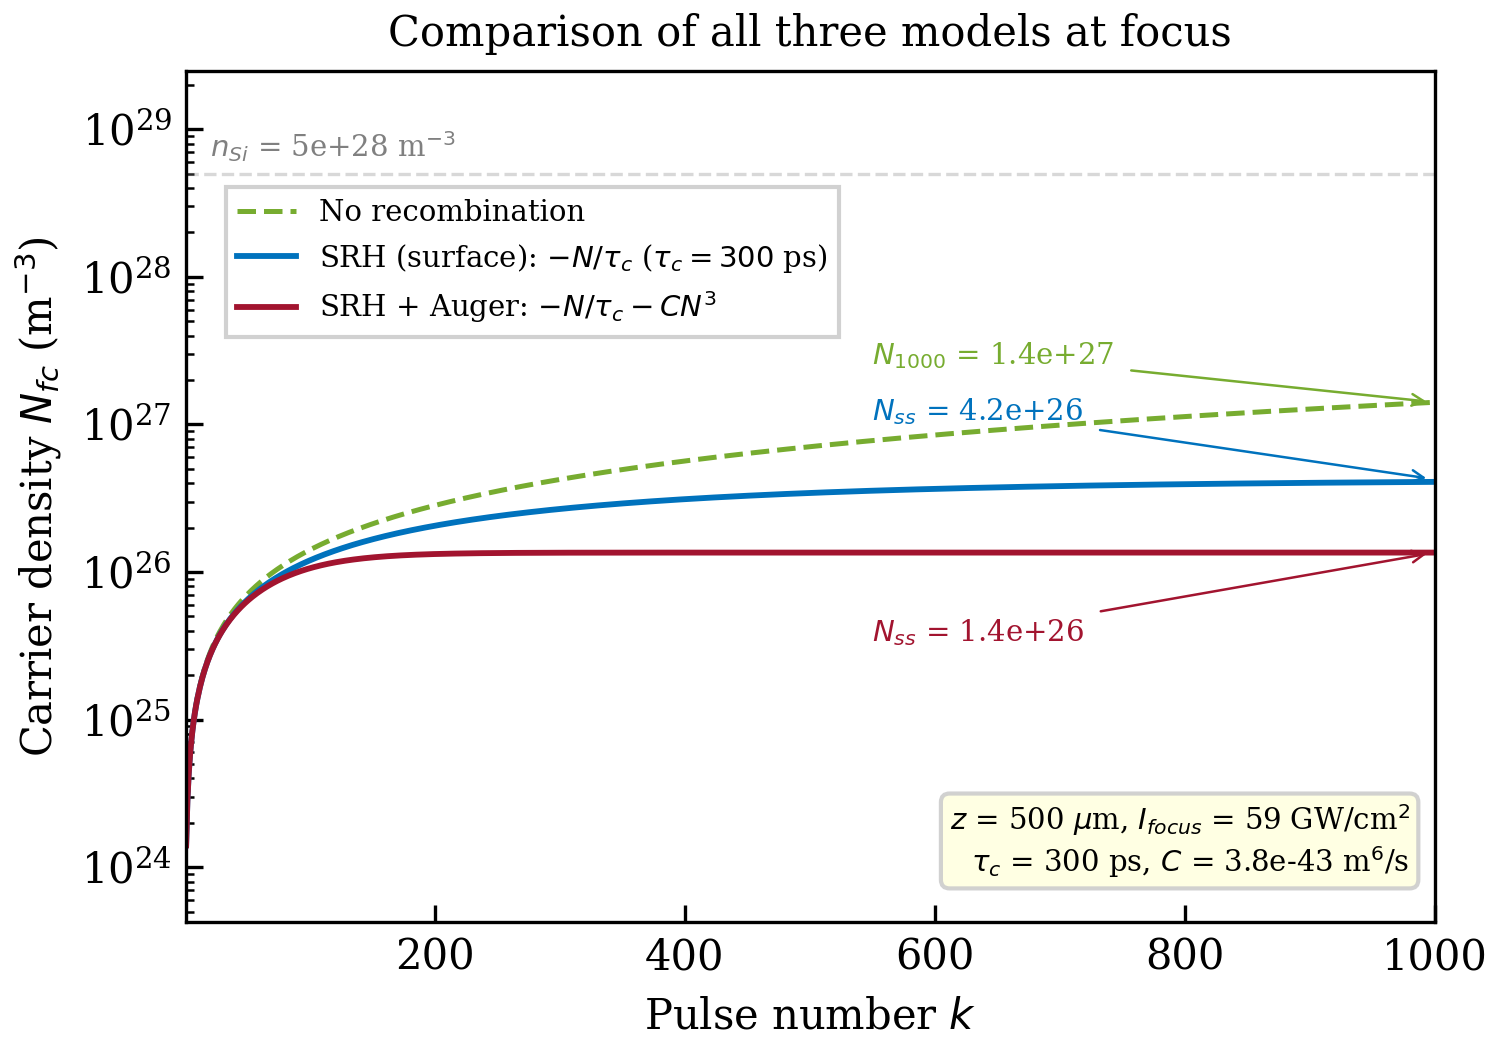
\includegraphics[width=0.85\textwidth]{figures_email/fig4_all_models.png}
\caption{Comparison of all three models at the focus ($z = \SI{500}{\mu m}$, $I_\text{focus} = \SI{59}{GW/cm^2}$): no recombination (dashed), SRH surface recombination only ($\tau_c = \SI{300}{ps}$), and SRH + Auger ($C = \SI{3.8e-31}{cm^6/s}$). Each mechanism progressively reduces the steady-state carrier density.}
\label{fig:all_models}
\end{figure}


\newpage
\section{Summary}

Three arguments establish the carrier dynamics:

\begin{enumerate}
\item \textbf{Without recombination}, carriers accumulate linearly (Eq.~6). At the focus, $N_{1000} = \SI{1.4e27}{m^{-3}}$ ($0.03 \times n_\text{Si}$).

\item \textbf{With SRH surface recombination} (Eq.~5, $\tau_c = \SI{300}{ps}$), the pulsed ODE gives a finite steady state: $N_\text{ss} = \SI{4.2e26}{m^{-3}}$ ($0.008 \times n_\text{Si}$) --- a $3.3\times$ reduction. The linear $N/\tau_c$ term represents SRH recombination at surface trap states \cite{li_textbook}, with $\tau_c = d/4S$, experimentally confirmed via $\tau \propto d$ in Si nanostructures \cite{grumstrup2014,li2023}. At their carrier densities (${\sim}\SI{e19}{cm^{-3}}$), the Auger lifetime $\tau_A = 1/CN^2 \approx \SI{26}{ns}$ is ${\sim}100\times$ longer than the measured surface lifetime, confirming Auger was negligible in those experiments.

\item \textbf{With SRH + Auger} ($N/\tau_c + CN^3$), the steady state drops to $N_\text{ss} = \SI{1.4e26}{m^{-3}}$ ($0.003 \times n_\text{Si}$) --- an additional $3\times$ reduction, or $10\times$ total from the no-recombination case. At our per-pulse carrier densities (${\sim}\SI{e20}{cm^{-3}}$), the Auger lifetime $\tau_A \approx \SI{16}{ps}$ is comparable to the inter-pulse spacing, making this channel significant.
\end{enumerate}

\begin{table}[h]
\centering
\begin{tabular}{@{}lcccc@{}}
\toprule
Model & $N_\text{ss}$ (m$^{-3}$) & $N_\text{ss} / n_\text{Si}$ & Reduction & Equation \\
\midrule
No recombination ($k=1000$) & $\SI{1.4e27}{}$ & $0.03$ & $1\times$ (ref) & Eq.~\eqref{eq:linear} \\
SRH surface ($\tau_c = \SI{300}{ps}$) & $\SI{4.2e26}{}$ & $0.008$ & $3.3\times$ & Eq.~\eqref{eq:N0_exact} \\
SRH + Auger ($\tau_c + CN^3$) & $\SI{1.4e26}{}$ & $0.003$ & $10\times$ & Eq.~\eqref{eq:bernoulli_solution} \\
\bottomrule
\end{tabular}
\caption{Steady-state carrier density at the focus ($z = \SI{500}{\mu m}$, $I_\text{focus} = \SI{59}{GW/cm^2}$) for each model. The ``Reduction'' column shows the factor relative to the no-recombination case. Parameters: $\tau_c = \SI{300}{ps}$, $C = \SI{3.8e-31}{cm^6/s}$, $\mu_t = \SI{5650}{m^{-1}}$.}
\end{table}

\begin{thebibliography}{9}
\bibitem{grumstrup2014} E.~M.~Grumstrup \textit{et al.}, ``Ultrafast carrier dynamics of silicon nanowire ensembles,'' J.\ Phys.\ Chem.\ C \textbf{118}, 8634 (2014).
\bibitem{li2023} H.~Li \textit{et al.}, ``Nanoscale imaging of carrier dynamics in individual silicon nanowires,'' Nano Lett.\ \textbf{23}, 1445 (2023).
\bibitem{li_textbook} S.~S.~Li, \textit{Semiconductor Physical Electronics}, 2nd ed.\ (Springer, 2006), Ch.~6.
\bibitem{dziewior1977} J.~Dziewior and W.~Schmid, ``Auger coefficients for highly doped and highly excited silicon,'' Appl.\ Phys.\ Lett.\ \textbf{31}, 346 (1977).
\bibitem{yaroslavsky2002} A.~N.~Yaroslavsky \textit{et al.}, ``Optical properties of selected native and coagulated human brain tissues,'' Phys.\ Med.\ Biol.\ \textbf{47}, 2059 (2002).
\end{thebibliography}

\end{document}
